
\section{Results}
\label{sec:results}

We evaluate five LLM systems under the pinned Rector contract
(Section~\ref{sec:rector_eval}), scoring only \texttt{Rector\textbackslash Php*}
rules. The primary outcome is all files weighted discharge,
$\rho_w^{\mathrm{all}}$. We interpret contract scores jointly with syntax,
preservation, loadability, and PHPCompatibility diagnostics.

\paragraph*{Overview}
Figure~\ref{fig:model_overview} highlights three properties of contract progress under the pinned policy.. First, PCE reveals
substantial variation in discharged upgrade work, with weighted discharge
from 30.53\% to 72.80\%
(Table~\ref{tab:contract_discharge_summary}). Second, residual work
concentrates in PHP~8.x families
(Table~\ref{tab:php_family_discharge}). Third, contract progress does not
subsume robustness: higher discharge can still coincide with syntax
failures, reduced preservation, and new loadability regressions
(Tables~\ref{tab:syntax_model_results},
\ref{tab:runtime_slice_results}). Agreement with PHPCompatibility is
therefore informative, but incomplete
(Table~\ref{tab:phpcompat_validation}).

% =================================================================
%  TABLE 1 — CONTRACT DISCHARGE SUMMARY
% =================================================================
\begin{table*}[t]
\centering
\caption{Obligation discharge under the pinned contract.
  Weighted $\rho_w^{\mathrm{all}}$ and Discharged use all-files scoring;
  remaining columns are computed on analyzable migrated files only.}
\label{tab:contract_discharge_summary}
\setlength{\tabcolsep}{4pt}
\renewcommand{\arraystretch}{1.18}
\resizebox{\textwidth}{!}{%
\begin{tabular}{%
  L{3.6cm}
  R{1.6cm}@{\hspace{4pt}}
  R{1.8cm}@{\hspace{4pt}}
  R{1.4cm}@{\hspace{4pt}}
  R{1.6cm}@{\hspace{4pt}}
  R{1.4cm}@{\hspace{4pt}}
  R{1.5cm}@{\hspace{4pt}}
  R{1.1cm}%
}
\arrayrulecolor{hdrBlue}
\toprule[1.5pt]
\tophdr{System} &
\tophdr{Mean $\rho$ (\%)} &
\tophdr{Wtd $\rho_w^{\mathrm{all}}$ (\%)} &
\tophdr{Dischgd} &
\tophdr{Post trig $R$} &
\tophdr{Introed} &
\tophdr{Ctr-clean} &
\tophdr{$\rho_i{<}50\%$} \\
\midrule[1pt]
% --- Reference -------------------------------------------------
\rowcolor{rowA}
\refrow{Rector (reference)} &
\refrow{98.55} & \refrow{98.43} & \refrow{503} &
\refrow{17}    & \refrow{9}    & \refrow{89}  & \refrow{0} \\
\midrule[0.4pt]
% --- LLMs ------------------------------------------------------
\rowcolor{rowB}
Gemini 2.5 Pro               & 77.11 & 72.80 & 372 & 140 & 21 & 19 & 3  \\
\rowcolor{rowA}
GPT-5 Codex                         & 71.35 & 58.12 & 297 & 151 & 20 & 15 & 12 \\
\rowcolor{rowB}
Gemini 2.5 Flash                    & 62.32 & 53.42 & 273 & 203 & 17 & 13 & 24 \\
\rowcolor{rowA}
Claude Sonnet 4 \scriptsize(05-14)  & 56.97 & 53.23 & 272 & 244 & 17 &  6 & 33 \\
\rowcolor{rowB}
Llama 3.3 70B Instruct      & 34.21 & 30.53 & 156 & 347 & 18 & 2 & 66 \\
\bottomrule[1.5pt]
\end{tabular}}
{\scriptsize\emph{Note.}
  Analyzable file counts: Rector 100, Claude 97, Gemini Flash 91,
  Gemini Pro 97, GPT-5 Codex 88, Llama 95.}
\end{table*}

% =================================================================
%  FIGURE — Model overview  (placed right after summary table)
% =================================================================
\begin{figure*}[t]
\centering
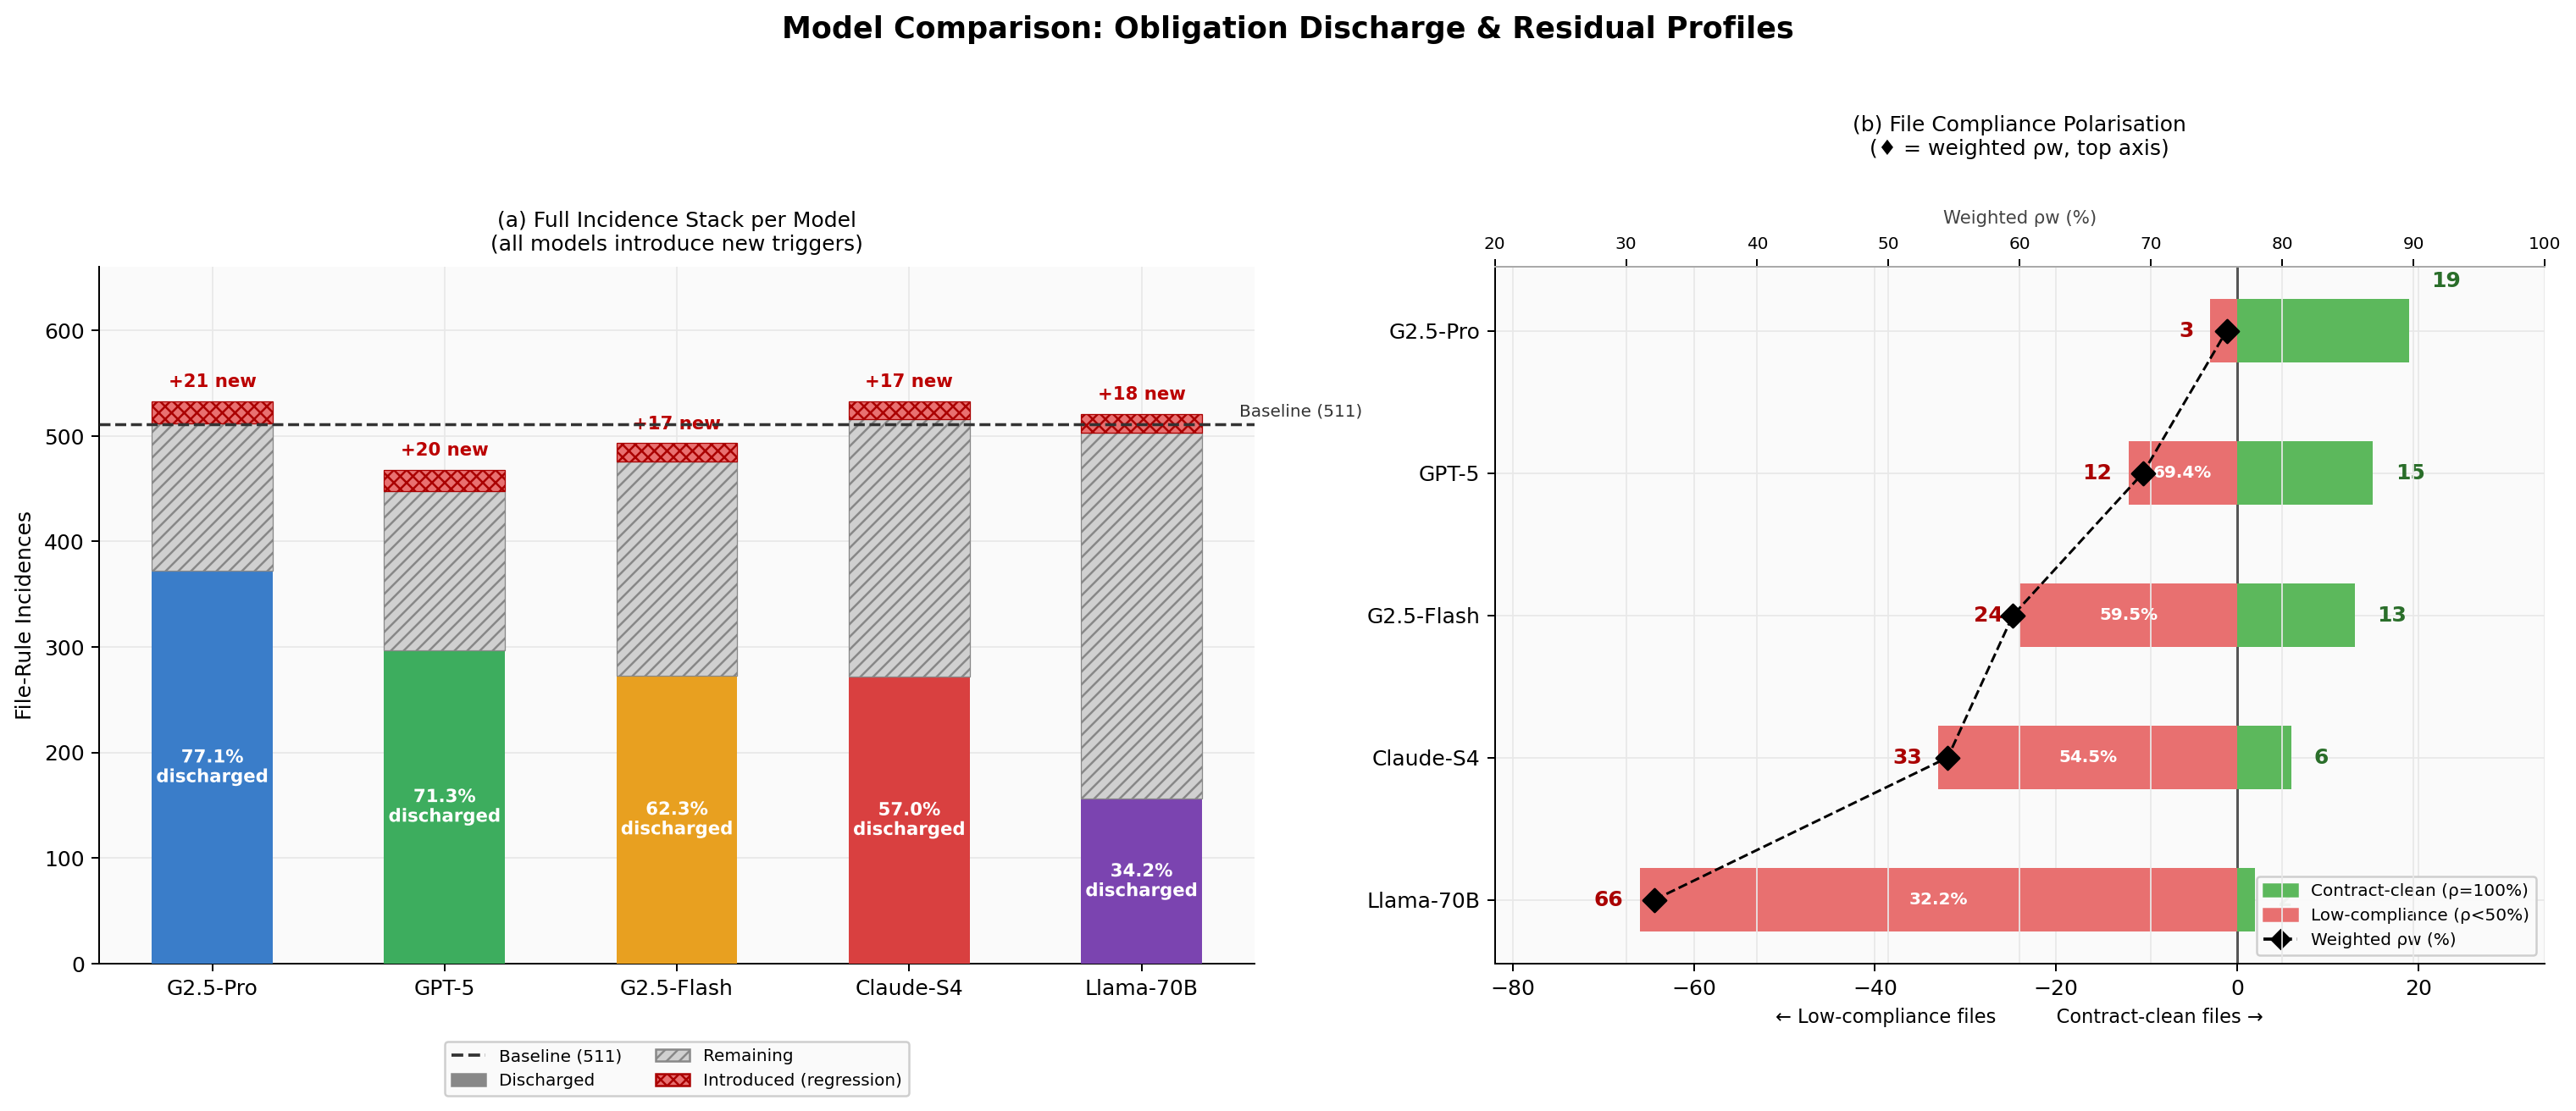
\includegraphics[width=\textwidth]{images/fig_models.png}
\caption{Pinned-contract compliance profiles across models.
  Bars show discharged and remaining obligations;
  auxiliary indicators summarise patch-volume closure and
  the concentration of remaining work.}
\label{fig:model_overview}
\end{figure*}


% =================================================================
%  SUBSECTION RQ1
% =================================================================
\subsection{RQ1: Migration progress under the pinned contract}
\label{sec:overall_results}

PCE reveals substantial variation in discharged and residual upgrade work
under a common all files denominator. Across 511 baseline file rule type
incidences, the contract aligned reference baseline (\emph{Rector applied})
discharges 503, yielding $\rho_w^{\mathrm{all}}=98.43\%$
(Table~\ref{tab:contract_discharge_summary}). This provides a strong,
though not perfect, reference point under the present ruleset.

For the LLM systems, weighted discharge ranges from 30.53\% to 72.80\%, with
2 to 19 contract clean files
(Table~\ref{tab:contract_discharge_summary}). Every system also introduces
new rule type incidences on analyzable migrated files. PCE therefore
separates discharged work, residual work, and newly introduced contract
visible regressions.


% =================================================================
%  SUBSECTION RQ2
% =================================================================
\subsection{RQ2: Resistant rules and migration demand}
\label{sec:size_results}

The remaining obligation space is structured rather than diffuse. Contract
progress declines as migration demand increases: discharge is lower on
larger files and on files with more baseline obligations
(Tables~\ref{tab:size_bin_discharge}, \ref{tab:correlation_results}).
Patch closure shows the same pattern, with unresolved work often
concentrated in a small number of files
(Table~\ref{tab:patch_closure},
Figure~\ref{fig:patch_concentration}).

Residual work is concentrated most clearly in PHP~8.x families
(Table~\ref{tab:php_family_discharge}). Rule level results show recurring
bottlenecks such as \texttt{NullToStrictStringFuncCallArg} and
\texttt{AddOverrideAttribute}, alongside introduced triggers such as
\texttt{ReadOnlyProperty}
(Table~\ref{tab:resistant_rules}). The main value of these results is
diagnostic: PCE localizes where automated migration remains least reliable
under a fixed policy.





% --- TWO side-by-side tables: size-bin discharge + patch closure --
\begin{table*}[t]
\centering
% ---- subtable A : size-bin discharge ----
\begin{minipage}[t]{0.56\textwidth}
\centering
\caption{Mean discharge (\%) by file-size bin .
  Parentheses: discharged / total incidences.}
\label{tab:size_bin_discharge}
\setlength{\tabcolsep}{4pt}
\renewcommand{\arraystretch}{1.18}
\resizebox{\linewidth}{!}{%
\begin{tabular}{L{3.0cm}C{1.8cm}C{1.8cm}C{1.7cm}C{2.0cm}}
\arrayrulecolor{hdrBlue}
\toprule[1.5pt]
\tophdr{Model} & \tophdr{Small} & \tophdr{Medium} & \tophdr{Large} & \tophdr{X-Large} \\
\midrule[1pt]
\rowcolor{rowA}
Gemini 2.5 Pro   & 77.6 {\tiny(77/99)} & 83.8 {\tiny(136/162)} & 74.8 {\tiny(105/141)} & 60.6 {\tiny(54/89)}  \\
\rowcolor{rowB}
GPT-5 Codex             & 75.9 {\tiny(76/99)}  & 75.9 {\tiny(111/146)} & 66.6 {\tiny(86/130)} & 45.1 {\tiny(24/53)}  \\
\rowcolor{rowA}
Gemini 2.5 Flash        & 71.5 {\tiny(70/99)}  & 67.0 {\tiny(104/153)} & 51.2 {\tiny(67/131)} & 41.8 {\tiny(32/76)}  \\
\rowcolor{rowB}
Claude Sonnet 4         & 65.8 {\tiny(60/91)}  & 69.3 {\tiny(111/158)} & 41.5 {\tiny(63/146)} & 38.3 {\tiny(38/104)} \\
\rowcolor{rowA}
Llama 3.3 70B   & 37.8 {\tiny(35/93)}  & 42.7 {\tiny(71/162)}  & 28.5 {\tiny(40/140)} & 11.9 {\tiny(10/90)}  \\
\bottomrule[1.5pt]
\end{tabular}}
\end{minipage}
\hfill
% ---- subtable B : patch closure ----
\begin{minipage}[t]{0.41\textwidth}
\centering
\caption{Patch-volume closure under the pinned contract (localization proxy).}
\label{tab:patch_closure}
\setlength{\tabcolsep}{4pt}
\renewcommand{\arraystretch}{1.18}
\resizebox{\linewidth}{!}{%
\begin{tabular}{L{2.8cm}C{1.3cm}C{1.3cm}C{1.4cm}R{2.0cm}}
\arrayrulecolor{hdrBlue}
\toprule[1.5pt]
\tophdr{System} & \tophdr{WDC} & \tophdr{MFDC} & \tophdr{Top-5} & \tophdr{Rem. lines} \\
\midrule[1pt]
\rowcolor{rowA}
\refrow{Rector (ref.)} & \refrow{95.1} & \refrow{98.2} & \refrow{91.4} & \refrow{1{,}109} \\
\midrule[0.4pt]
\rowcolor{rowB}
Gemini 2.5 Pro  & 71.9  & 76.9  & 50.7          & 5{,}826  \\
\rowcolor{rowA}
GPT-5 Codex            & 67.5         & 69.9         & 36.5   & 5{,}074  \\
\rowcolor{rowB}
Gemini 2.5 Flash       & 60.7         & 64.8         & 43.5          & 7{,}620  \\
\rowcolor{rowA}
Claude Sonnet 4        & 57.8         & 62.8         & 40.3          & 9{,}411  \\
\rowcolor{rowB}
Llama 3.3 70B  & 36.7 & 42.3 & 39.4          & 12{,}342 \\
\bottomrule[1.5pt]
\end{tabular}}
\end{minipage}
\end{table*}

% =================================================================
%  FIGURE — Patch concentration  (inline with RQ2 text)
% =================================================================
\begin{figure}[t]
\centering
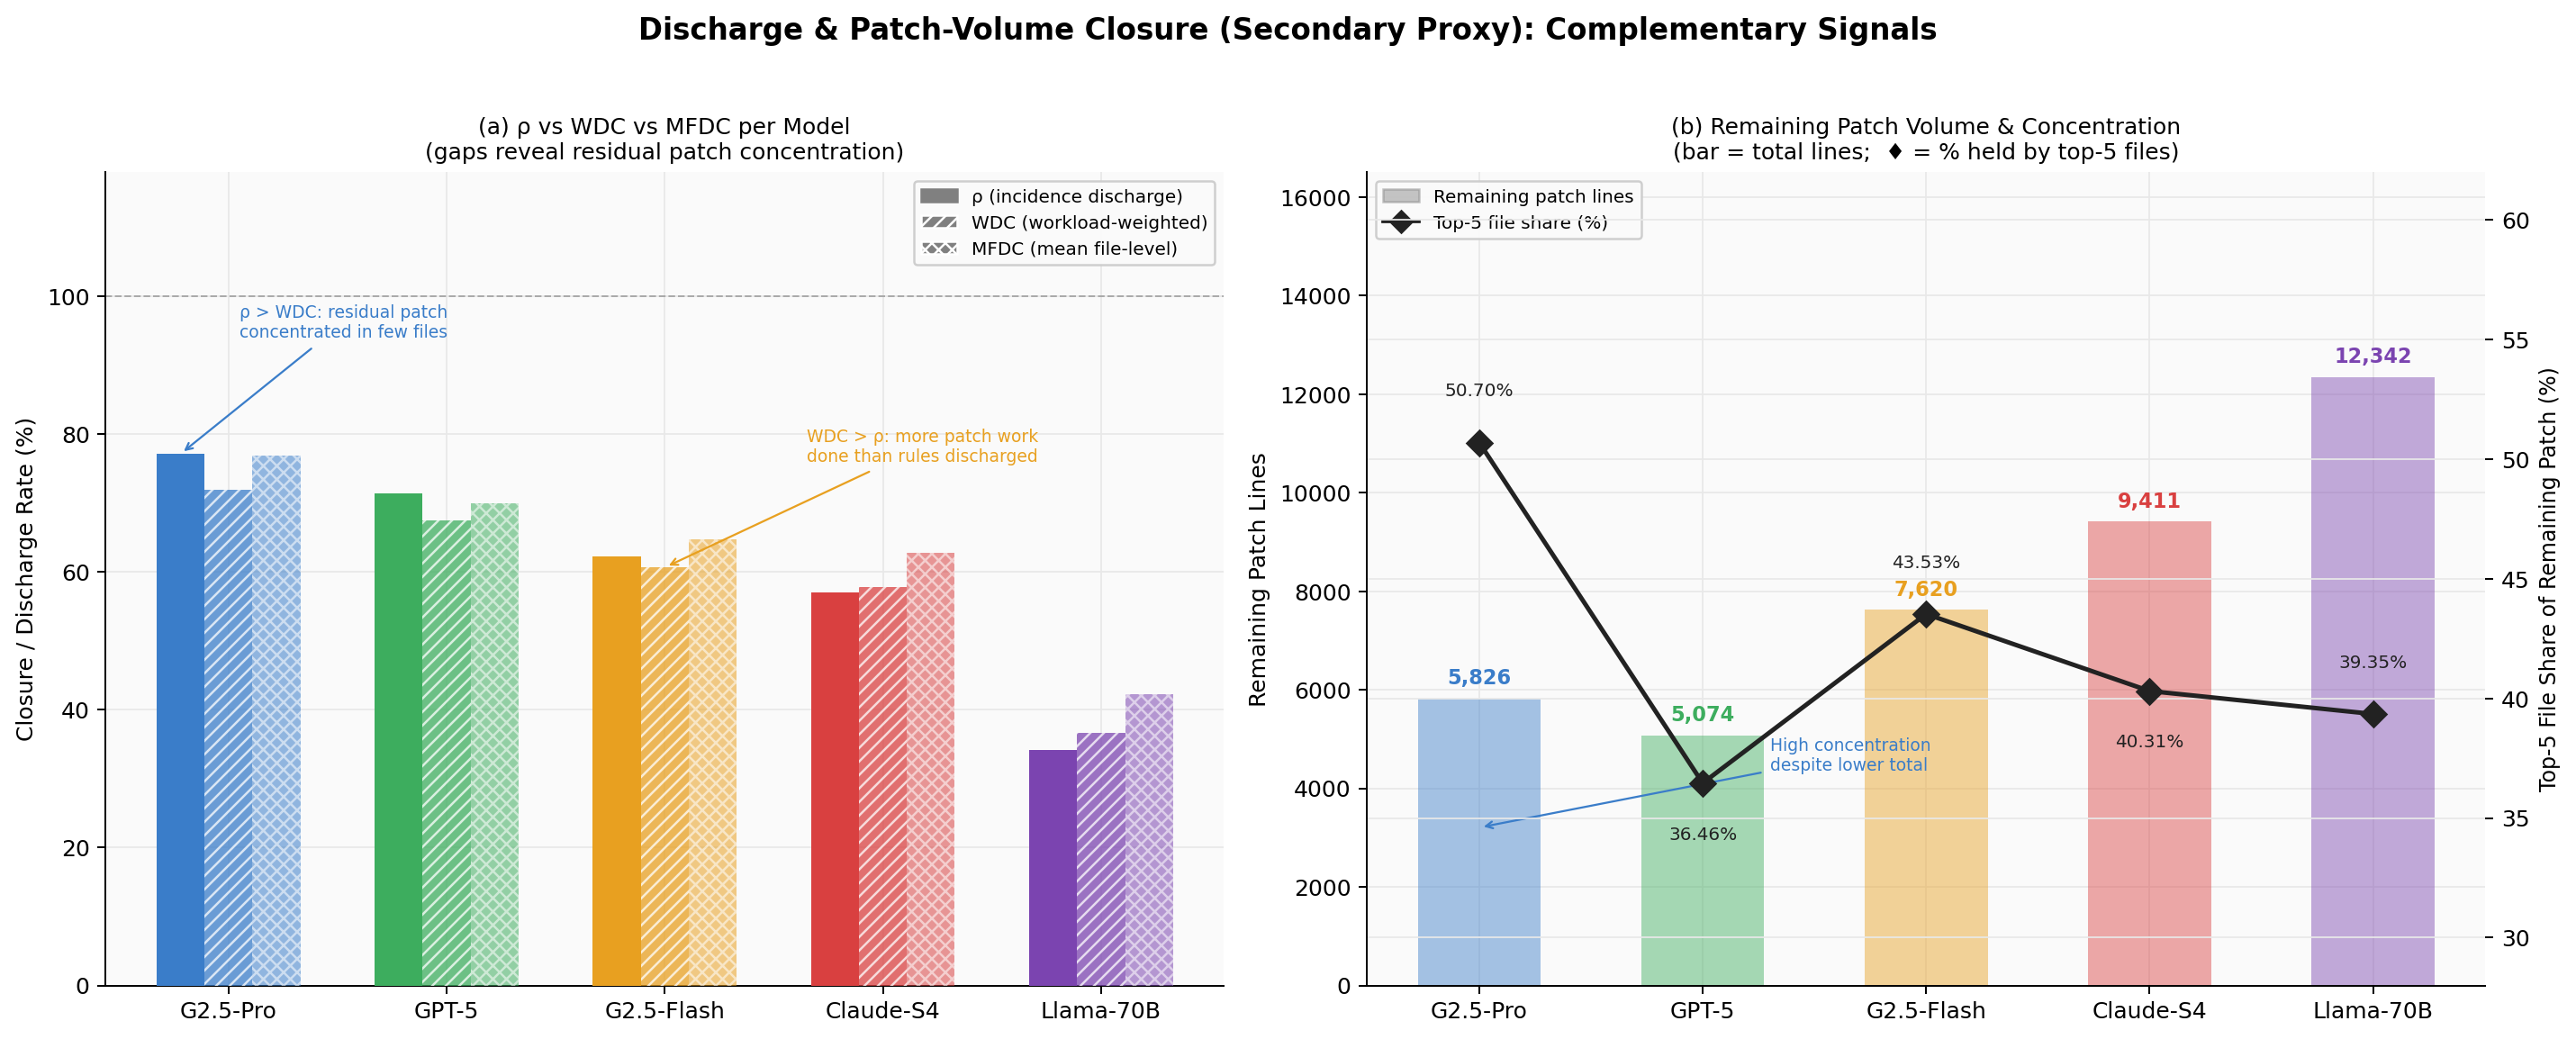
\includegraphics[width=\columnwidth]{images/fig_patch.png}
\caption{Remaining patch volume and concentration across models.
  Bars show total remaining patch lines;
  markers show the share concentrated in the top files.}
\label{fig:patch_concentration}
\end{figure}



% --- TWO side-by-side tables: PHP-family discharge + correlation --
\begin{table*}[t]
\centering
\begin{minipage}[t]{0.54\textwidth}
\centering
\caption{Discharged obligations by PHP family (analyzable files only).}
\label{tab:php_family_discharge}
\setlength{\tabcolsep}{4pt}
\renewcommand{\arraystretch}{1.18}
\resizebox{\linewidth}{!}{%
\begin{tabular}{L{3.2cm}C{2.6cm}C{2.6cm}C{2.6cm}}
\arrayrulecolor{hdrBlue}
\toprule[1.5pt]
\tophdr{Model} & \tophdr{PHP 5.x} & \tophdr{PHP 7.x} & \tophdr{PHP 8.x} \\
\midrule[1pt]
\rowcolor{rowA}
Gemini 2.5 Pro  & 143/149 (95.97\%) & 114/126 (90.48\%) & 115/216 (53.24\%) \\
\rowcolor{rowB}
GPT-5 Codex            & 126/133 (94.74\%)        & 88/106 (83.02\%)         & 83/189 (43.92\%)  \\
\rowcolor{rowA}
Gemini 2.5 Flash       & 116/137 (84.67\%)        & 97/120 (80.83\%)         & 60/202 (29.70\%)  \\
\rowcolor{rowB}
Claude Sonnet 4        & 109/150 (72.67\%)        & 92/129 (71.32\%)         & 71/220 (32.27\%)  \\
\rowcolor{rowA}
Llama 3.3 70B  & 87/145 (60.00\%) & 53/125 (42.40\%) & 16/215 (7.44\%)  \\
\bottomrule[1.5pt]
\end{tabular}}
\end{minipage}
\hfill
\begin{minipage}[t]{0.42\textwidth}
\centering
\caption{Pearson correlation between demand proxies and type-level
  discharge on each model's analyzable migrated files.}
\label{tab:correlation_results}
\setlength{\tabcolsep}{4pt}
\renewcommand{\arraystretch}{1.18}
\resizebox{\linewidth}{!}{%
\begin{tabular}{L{3.4cm}C{2.0cm}C{2.0cm}}
\arrayrulecolor{hdrBlue}
\toprule[1.5pt]
\tophdr{Model} & \tophdr{$r(\mathrm{LOC},\rho_i)$} & \tophdr{$r(O_i,\rho_i)$} \\
\midrule[1pt]
\rowcolor{rowA}
Gemini 2.5 Flash       & $-$0.453 & $-$0.300 \\
\rowcolor{rowB}
Gemini 2.5 Pro         & $-$0.405 & $-$0.212 \\
\rowcolor{rowA}
GPT-5 Codex            & $-$0.337 & $-$0.236 \\
\rowcolor{rowB}
Claude Sonnet 4        & $-$0.459 & $-$0.267 \\
\rowcolor{rowA}
Llama 3.3 70B          & $-$0.356 & $-$0.204 \\
\bottomrule[1.5pt]
\end{tabular}}
\end{minipage}
\end{table*}

% --- Resistant rules table (full width) --------------------------
\begin{table*}[t]
\centering
\caption{Most resistant Rector upgrade rules across models (file-level trigger breadth).
  \emph{Orig.}\ = benchmark files in which the rule triggers.
  For Orig.\,$>$0: \% of file-level triggers discharged.
  For Orig.\,=\,0: introduced file-level triggers ($+k$).}
\label{tab:resistant_rules}
\setlength{\tabcolsep}{4pt}
\renewcommand{\arraystretch}{1.18}
\resizebox{\textwidth}{!}{%
\begin{tabular}{%
  L{3.6cm}          % Rule
  C{0.9cm}          % PHP ver
  L{4.4cm}          % Challenge
  C{1.0cm}          % Orig
  C{1.3cm}          % Pro
  C{1.3cm}          % Flash
  C{1.3cm}          % GPT-5
  C{1.3cm}          % Claude
  C{1.3cm}%         % LLaMA
}
\arrayrulecolor{hdrBlue}
\toprule[1.5pt]
\tophdr{Rule} &
\tophdr{PHP} &
\tophdr{Migration Challenge} &
\tophdr{Orig.} &
\tophdr{Pro} &
\tophdr{Flash} &
\tophdr{GPT-5} &
\tophdr{Claude} &
\tophdr{LLaMA} \\
\midrule[1pt]
% --- group header -----------------------------------------------
\multicolumn{9}{l}{\subhdr{\quad Type strictness \& null-safety}} \\
\rowcolor{rowA}
\texttt{\small NullToStrict\-Func\-Call\-Arg} & 8.1 &
  Null-safety across non-local flow & 81 & 27 & 32 & 48 & 11 & 14 \\
\rowcolor{rowB}
\texttt{\small Stringable\-For\-ToString}      & 8.0 &
  Interface decl.\ for \texttt{\_\_toString()} &  8 & 13 & 13 &  0 &  0 &  0 \\
\midrule[0.4pt]
\multicolumn{9}{l}{\subhdr{\quad Modern callable \& attribute syntax (near-zero discharge)}} \\
\rowcolor{rowA}
\texttt{\small FirstClass\-Callable}           & 8.1 &
  Callable vs.\ string-literal ambiguity & 13 & 31 & 23 & 15 &  8 &  8 \\
\rowcolor{rowB}
\texttt{\small AddOverride\-Attribute}         & 8.3 &
  Cross-file hierarchy reasoning         &  7 & 29 & 14 & 29 & 14 & 14 \\
\rowcolor{rowA}
\texttt{\small AddType\-To\-Const}             & 8.3 &
  Type decls.\ requiring global inference &  0 & +5 & +1 & +1 & +2 & +1 \\
\midrule[0.4pt]
\multicolumn{9}{l}{\subhdr{\quad Introduced ``modern'' constructs (over-eager / regression risk)}} \\
\rowcolor{rowB}
\texttt{\small ReadOnly\-Property}             & 8.1 &
  Single-assignment detection (FP risk)  &  0 & +8 & +4 & +4 & +5 & +9 \\
\bottomrule[1.5pt]
\end{tabular}}
\end{table*}


% =================================================================
%  SUBSECTION RQ3 — Validity, preservation, loadability
% =================================================================
\subsection{RQ3: Contract progress and complementary diagnostics}
\label{sec:syntax_and_structure}

Contract progress and robustness align only partially
(Figure~\ref{fig:robustness}). All LLM systems introduce new syntax
failures
(Table~\ref{tab:syntax_model_results}), showing that substantial discharge
does not by itself guarantee a parsable result set.

Structural diagnostics add a second qualification
(Table~\ref{tab:completeness_model_results}). Signature stability remains
high, but deeper preservation varies more noticeably. The loadability
sentinel shows the same partial alignment: new failures on the execution
slice range from 14.5\% to 32.7\%
(Table~\ref{tab:runtime_slice_results}). PCE is therefore informative about
policy grounded migration progress, but it must be read with orthogonal
diagnostics.

% --- TWO side-by-side tables: syntax + loadability ---------------
\begin{table*}[t]
\centering
\begin{minipage}[t]{0.50\textwidth}
\centering
\caption{Syntax validity (\texttt{php -l}, PHP 8.3) over 100 files.
  \textbf{New} = hard regressions (Pass$\to$Fail).
  NR-valid = Both valid + Fixed.}
\label{tab:syntax_model_results}
\setlength{\tabcolsep}{4pt}
\renewcommand{\arraystretch}{1.18}
\resizebox{\linewidth}{!}{%
\begin{tabular}{L{3.2cm}C{0.9cm}C{1.2cm}C{1.1cm}C{1.5cm}C{1.5cm}C{1.3cm}}
\arrayrulecolor{hdrBlue}
\toprule[1.5pt]
\tophdr{System} &
\tophdr{New$\downarrow$} &
\tophdr{Migr Err} &
\tophdr{Fixed$\uparrow$} &
\tophdr{Both valid} &
\tophdr{NR-valid$\uparrow$} &
\tophdr{Orig Err} \\
\midrule[1pt]
\rowcolor{rowA}
\refrow{Rector (ref.)} & \refrow{1} & \refrow{1} & \refrow{9} & \refrow{90} & \refrow{99} & \refrow{9} \\
\midrule[0.4pt]
\rowcolor{rowB}
Gemini 2.5 Pro  & 11 & 13 & 7 & 80 & 87 & 9 \\
\rowcolor{rowA}
Claude Sonnet 4 & 11 & 12 & 8 & 80 & 88 & 9 \\
\rowcolor{rowB}
GPT-5 Codex            & 14 & 18 & 5 & 77 & 82 & 9 \\
\rowcolor{rowA}
Llama 3.3 70B          & 16 & 23 & 2 & 75 & 77 & 9 \\
\rowcolor{rowB}
Gemini 2.5 Flash & 18 & 20 & 7 & 73 & 80 & 9 \\
\bottomrule[1.5pt]
\end{tabular}}
\end{minipage}
\hfill
\begin{minipage}[t]{0.46\textwidth}
\centering
\caption{Loadability tripwire on the 55-file execution slice (\%).
  \textbf{Regress} = new failures (Pass$\to$Fail). $\rho$ = mean discharge.}
\label{tab:runtime_slice_results}
\setlength{\tabcolsep}{4pt}
\renewcommand{\arraystretch}{1.18}
\resizebox{\linewidth}{!}{%
\begin{tabular}{L{3.2cm}C{1.5cm}C{1.2cm}C{1.2cm}C{1.2cm}}
\arrayrulecolor{hdrBlue}
\toprule[1.5pt]
\tophdr{System} &
\tophdr{Regress$\downarrow$} &
\tophdr{Pass$\uparrow$} &
\tophdr{$\rho$} &
\tophdr{Other} \\
\midrule[1pt]
\rowcolor{rowA}
\refrow{Rector (ref.)}  & \refrow{12.7} & \refrow{83.6} & \refrow{98.3} & \refrow{3.6} \\
\midrule[0.4pt]
\rowcolor{rowB}
Claude Sonnet 4  & 14.5  & 80.0 & 57.0 & 5.5 \\
\rowcolor{rowA}
GPT-5 Codex             & 16.4  & 78.2 & 58.7 & 5.5 \\
\rowcolor{rowB}
Gemini 2.5 Pro          & 21.8  & 72.7 & 74.6 & 5.5 \\
\rowcolor{rowA}
Llama 3.3 70B           & 21.8  & 69.1 & 36.2 & 9.1 \\
\rowcolor{rowB}
Gemini 2.5 Flash& 32.7 & 60.0 & 53.5 & 7.3 \\
\bottomrule[1.5pt]
\end{tabular}}
\end{minipage}
\end{table*}

% --- Structural preservation (full width) -----------------------
\begin{table*}[t]
\centering
\caption{Structural preservation and anti-gaming diagnostics over 100 files.
  Line/Func/Class/Struct are retention ratios ($>$100\% indicates expansion).
  Body/SigStab/TrivialStub/EmptyBody are computed on matched declarations (80/100).}
\label{tab:completeness_model_results}
\setlength{\tabcolsep}{4pt}
\renewcommand{\arraystretch}{1.18}
\resizebox{\textwidth}{!}{%
\begin{tabular}{%
  L{3.4cm}
  C{1.4cm}C{1.3cm}C{1.3cm}C{1.3cm}C{1.3cm}C{1.4cm}C{1.5cm}C{1.5cm}%
}
\arrayrulecolor{hdrBlue}
\toprule[1.5pt]
\tophdr{System} &
\tophdr{Line (\%)} &
\tophdr{Func (\%)} &
\tophdr{Class (\%)} &
\tophdr{Struct (\%)} &
\tophdr{Body (\%)} &
\tophdr{SigStab} &
\tophdr{Trivial\-Stub} &
\tophdr{Empty\-Body} \\
\midrule[1pt]
\rowcolor{rowA}
\refrow{Rector (ref.)}  &  \refrow{98.87} &  \refrow{99.91} & \refrow{100.00} & \refrow{97.69} & \refrow{95.73} & \refrow{1.000} & \refrow{0.082} & \refrow{0.038} \\
\midrule[0.4pt]
\rowcolor{rowB}
Claude Sonnet 4         &  97.37 & 102.16 & 100.00 & 95.23 & 91.95 & 0.996 & 0.123 & 0.035 \\
\rowcolor{rowA}
GPT-5 Codex             & 105.40 &  96.03 &  99.00 & 94.02 &       93.16  &       0.988  & 0.116 & 0.027 \\
\rowcolor{rowB}
Gemini 2.5 Flash        &  95.85 &  96.57 &  99.00 & 91.39 &       89.39  &       0.989  & 0.114 & 0.037 \\
\rowcolor{rowA}
Gemini 2.5 Pro   & 100.04 &  97.42 &  99.50 & 90.20 & 80.20 & 0.979 & 0.115 & 0.024 \\
\rowcolor{rowB}
Llama 3.3 70B           &  97.12 &  98.33 &  99.00 & 89.96 &       93.67  &       0.990  & 0.106 & 0.018 \\
\bottomrule[1.5pt]
\end{tabular}}
\end{table*}

% --- Robustness figure ------------------------------------------
\begin{figure*}[t]
\centering
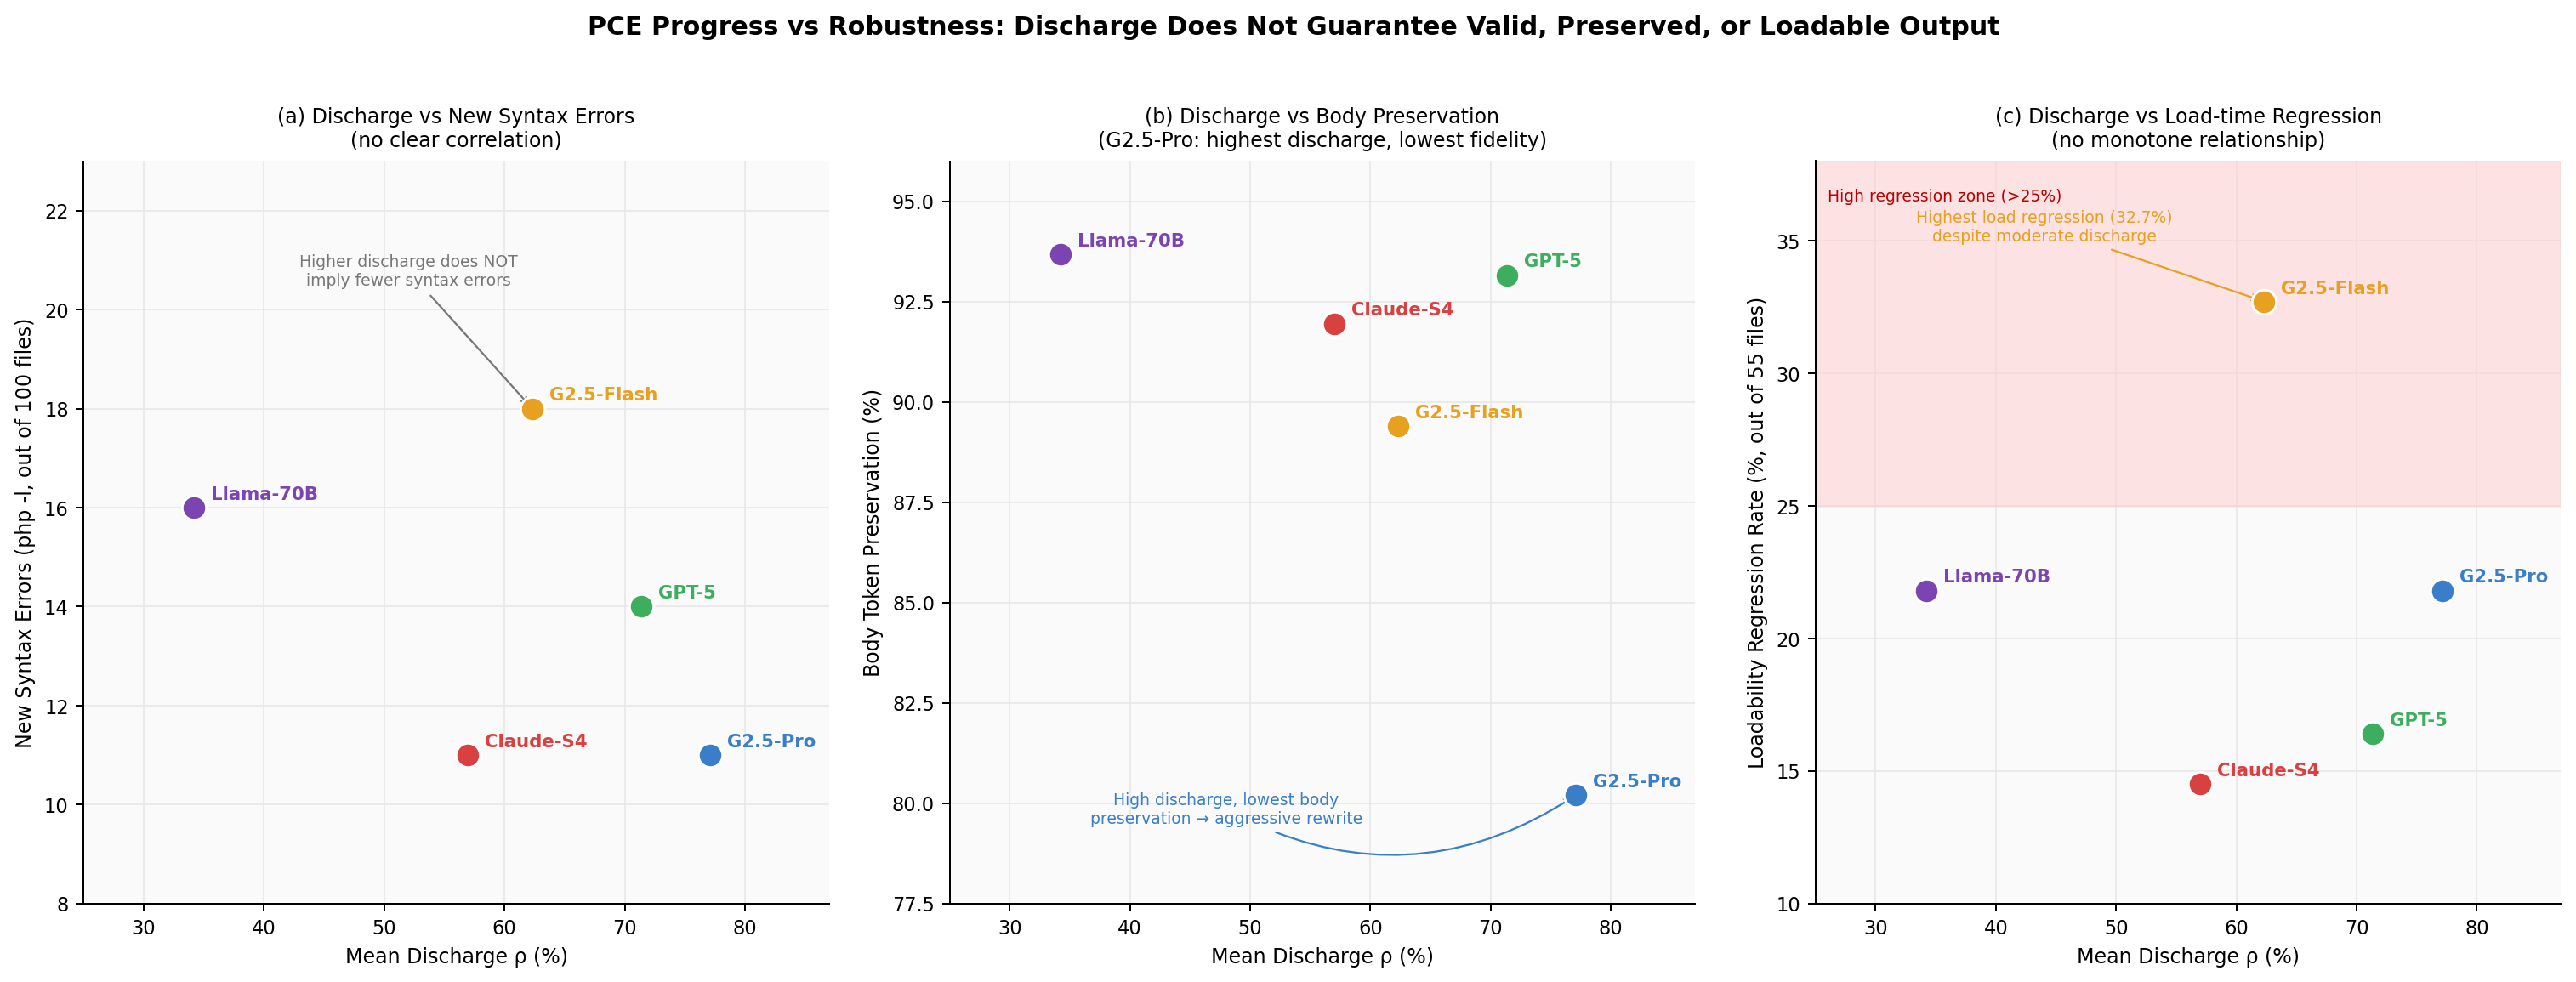
\includegraphics[width=\textwidth]{images/fig_validity.png}
\caption{Contract discharge versus robustness diagnostics across models.
  Higher contract compliance does not necessarily imply fewer syntax
  errors, stronger structural preservation, or better loadability.}
\label{fig:robustness}
\end{figure*}


% =================================================================
%  SUBSECTION RQ4 — PHPCompatibility
% =================================================================
\subsection{RQ4: Cross instrument triangulation with PHPCompatibility}
\label{sec:phpcompat_results}

PCE and PHPCompatibility provide related but non identical views of
migration progress
(Table~\ref{tab:phpcompat_validation}). Some systems improve under both
instruments, but the magnitude of improvement and the relative ordering do
not fully coincide.

This divergence is methodological rather than contradictory. PCE measures
discharged obligations under a pinned Rector contract, whereas
PHPCompatibility reports issues under an independent rule set. Read
together, they show that evaluation conclusions depend in part on the
instrument used.

% --- PHPCompatibility table (full width) ------------------------
\begin{table*}[t]
\centering
\caption{PHPCS+PHPCompatibility results (\texttt{testVersion=8.3}) with
  concentration diagnostics over 100 files.
  Issues = errors + warnings; Clean = zero-issue files;
  $\Delta$Issues relative to original benchmark.}
\label{tab:phpcompat_validation}
\setlength{\tabcolsep}{4pt}
\renewcommand{\arraystretch}{1.18}
\resizebox{\textwidth}{!}{%
\begin{tabular}{%
  L{3.2cm}
  R{1.3cm}@{\hspace{3pt}}
  R{1.4cm}@{\hspace{3pt}}
  R{1.1cm}@{\hspace{3pt}}
  R{1.1cm}@{\hspace{3pt}}
  R{1.4cm}@{\hspace{3pt}}
  R{1.0cm}@{\hspace{3pt}}
  R{1.2cm}@{\hspace{3pt}}
  L{2.8cm}@{\hspace{3pt}}
  R{1.2cm}%
}
\arrayrulecolor{hdrBlue}
\toprule[1.5pt]
\tophdr{System} &
\tophdr{Issues$\downarrow$} &
\tophdr{$\Delta$Issues} &
\tophdr{Err$\downarrow$} &
\tophdr{Warn$\downarrow$} &
\tophdr{Clean$\uparrow$} &
\tophdr{P95$\downarrow$} &
\tophdr{Top-5} &
\tophdr{Dom.\ code} &
\tophdr{Share} \\
\midrule[1pt]
\rowcolor{rowA}
\refrow{Original}          & \refrow{255} & \refrow{0}    & \refrow{45}  & \refrow{210} & \refrow{76 (76\%)} & \refrow{14} & \refrow{63.9\%} & \texttt{\scriptsize CurlyBraceAccess} & \refrow{56.1\%} \\
\rowcolor{rowB}
\refrow{Rector (ref.)}     & \refrow{48}  & \refrow{$-$207} & \refrow{27}  & \refrow{21}  & \refrow{88 (88\%)} & \refrow{3}  & \refrow{77.1\%} & \texttt{\scriptsize mysql\_removed}   & \refrow{43.8\%} \\
\midrule[0.6pt]
\rowcolor{rowA}
Gemini 2.5 Pro  & 10   & $-$245 & 9   & 1  & 97 (97\%) & 0 & 100.0\%& \texttt{\scriptsize mysql\_removed}   & 70.0\%  \\
\rowcolor{rowB}
Claude Sonnet 4        & 39          & $-$216          & 27         & 12        & 90 (90\%)        & 2        & 84.6\%         & \texttt{\scriptsize mysql\_removed}   & 53.8\%  \\
\rowcolor{rowA}
Gemini 2.5 Flash       & 139         & $-$116          & 125        & 14        & 88 (88\%)        & 2        & 93.5\%         & \texttt{\scriptsize this\_outside}    & 76.3\%  \\
\rowcolor{rowB}
GPT-5 Codex            & 181         & $-$74           & 172        &  9        & 91 (91\%)        & 1        & 97.8\%         & \texttt{\scriptsize this\_outside}    & 87.3\%  \\
\rowcolor{rowA}
Llama 3.3 70B  & 484 & $+$229  & 377& 107& 85 (85\%)& 6& 95.2\%         & \texttt{\scriptsize this\_outside}    & 71.5\%  \\
\bottomrule[1.5pt]
\end{tabular}}
\end{table*}


% =================================================================
%  SUMMARY
% =================================================================
\subsection{Summary}
\label{sec:tradeoffs}

Taken together, the results support the role of PCE as a policy grounded
measurement layer rather than a stand alone correctness signal. Under the
pinned contract, PCE reveals substantial variation in discharged migration
work, with unresolved obligations concentrated in PHP~8.x families.
Complementary diagnostics then delimit what that progress does and does not
imply about syntax, preservation, loadability, and independent
compatibility.